Philip Schäfers, Maximilian Sackel
\section*{a,b,c}
Zunächst werden die Daten eingelesen und die NaNs durch den Mittelwert bei values ersetzt und bei Strings durch Unknown. In der Challenge wurden die Strings dann in Pseudovariablen umgewandelt die den Wert True or False annehmen können. Somit bestitzen diese features eine Aussagekraft im Gegensatz zu der ersten Version.
Mittels fRegression werden die di Attribute mit der höchsten Korrelation zum target gesucht. Die feature mit den höchsten Korrelation sind den Plots zu entnehmen.
\begin{figure}
  \centering
  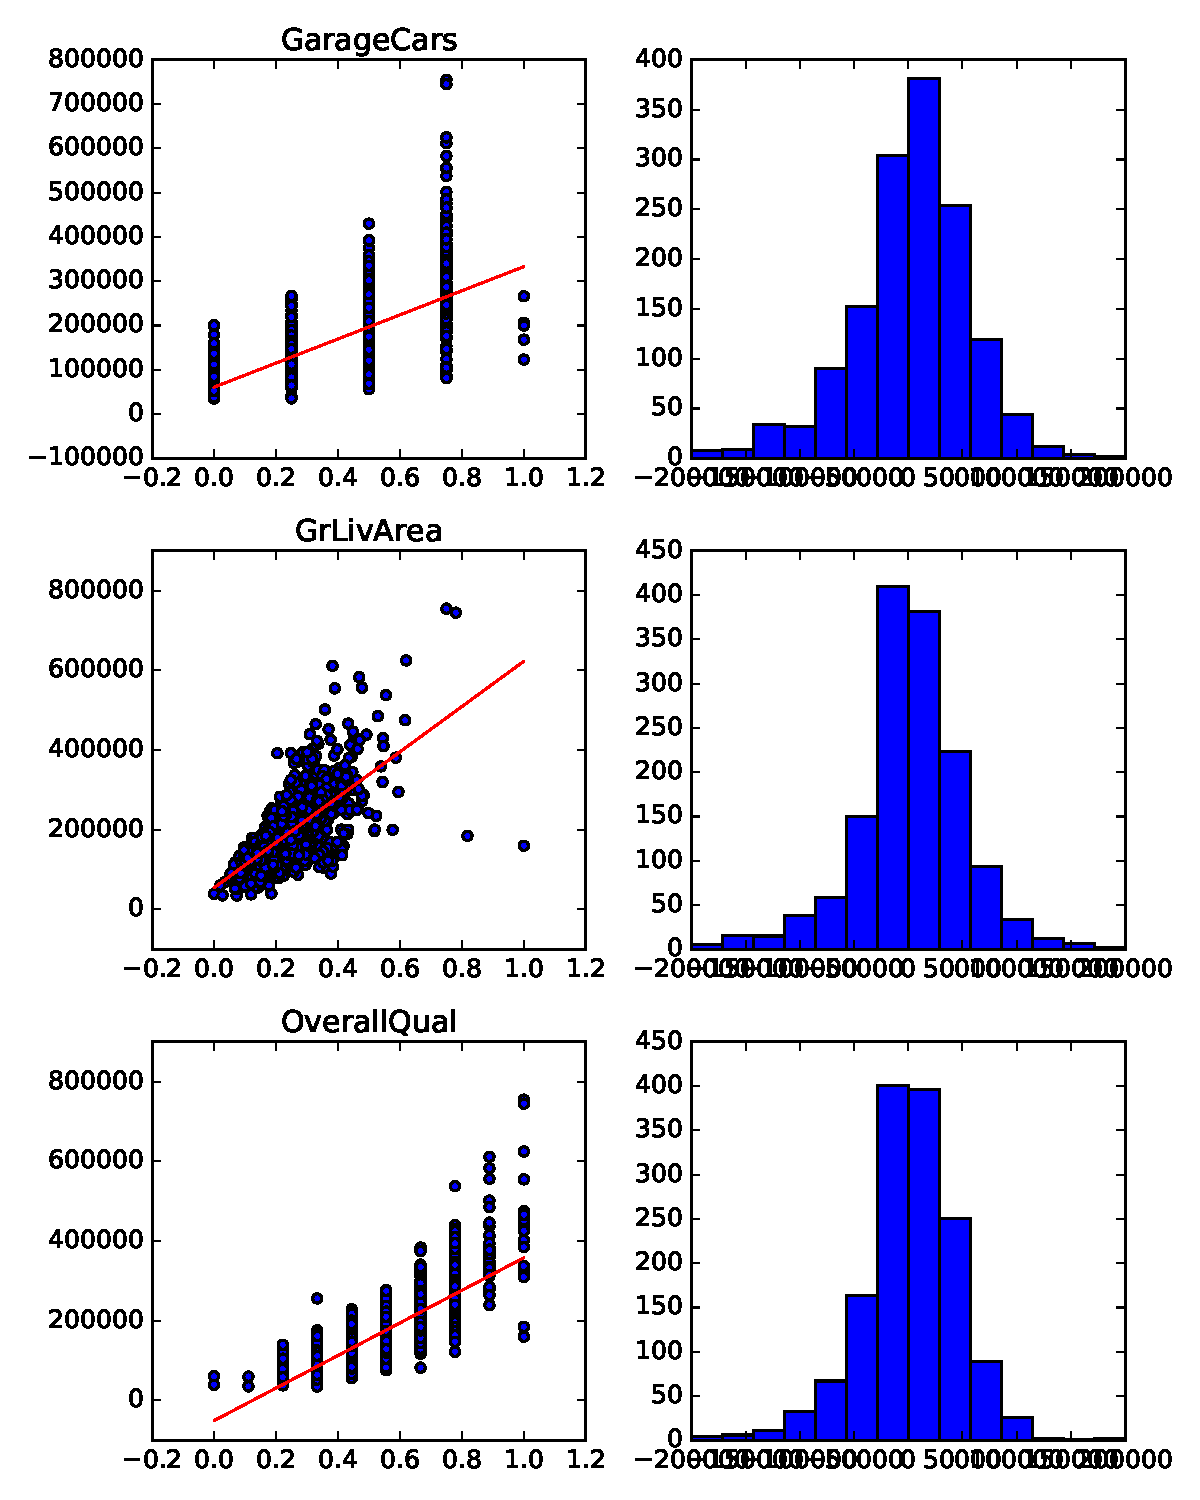
\includegraphics[height=8cm]{./Python/bundc.pdf}
  \caption{Regressiongrade und Abweichung vom Verkaufspreis}
\end{figure}
\section*{d}
In der Challenge wurde ein mix aus Random Forrest Regressor und Lasso genommen um eine höhere genauigkeit zu erlangen. Dabei wurde jedoch der Forrest nicht weiter aus Zeitmangel trainiert.
